\subsection{Irrational Numbers and Real Numbers}
Of the numbers on the number line, not all are rational.
\begin{definition}[Real numbers]
A number that cannot be written as a fraction is called \term{irrational}. The rational numbers combined with the irrational numbers make up the \term{real numbers}, represented by the symbol $\mathbb{R}$. The real numbers make up all of what we think of as ``numbers.''
\end{definition}
What are these irrational numbers, anyway?
\begin{example}
The number $0.10110011100011110000\dots$ is irrational. This decimal does not \makeblank[1in] or \makeblank[1in].
\end{example}
\begin{example}
The number $\sqrt{2}$ is irrational. In fact, for any whole number $n$, $\sqrt{n}$ is either a whole number or irrational.
\end{example}
\begin{example}There are also some numbers that are defined to work in formulas that turn out to be irrational, such as the number $\pi$, which is defined to work in the formula $C=2\pi r$ for the \makeblank of a circle.
\end{example}
\begin{example}
Which of these numbers are Whole numbers? Integers? Rational numbers?
\begin{itemize}
\item $-2.3$ \checkbox{Rational Number} \checkbox{Irrational Number} \checkbox{Real Number}
\makeblanknew
\item $\sqrt{5}$ \checkbox{Rational Number} \checkbox{Irrational Number} \checkbox{Real Number}
\makeblanknew
\item $\sqrt{9}$ \checkbox{Rational Number} \checkbox{Irrational Number} \checkbox{Real Number}
\makeblanknew
\item $\pi$ \checkbox{Rational Number} \checkbox{Irrational Number} \checkbox{Real Number}
\makeblanknew
\end{itemize}
\end{example}
We can organize all of our number sets:
\begin{center}
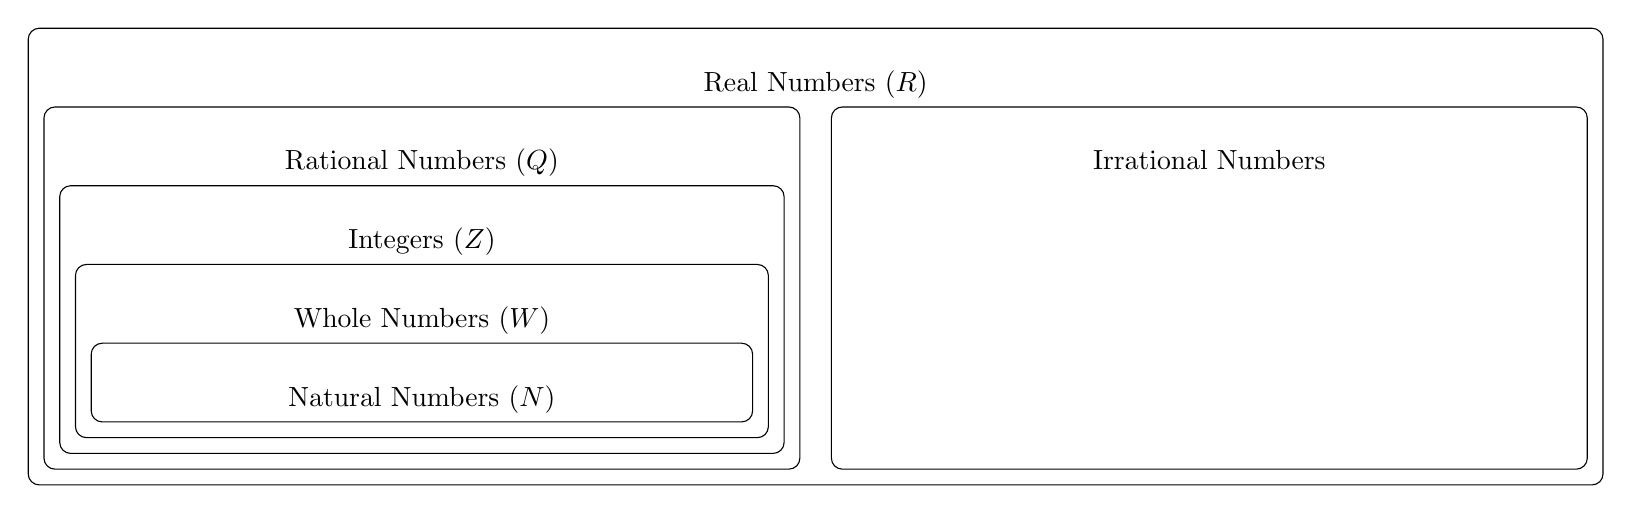
\begin{tikzpicture}
\foreach \x in {1,2,3,4}
	\draw[rounded corners] (-4-\x/5,0.2-\x/5) rectangle (4+\x/5,\x);
\draw (0,0.2) node[anchor=base] {Natural Numbers ($\mathbb{N}$)};
\draw (0,1.2) node[anchor=base] {Whole Numbers ($\mathbb{W}$)};
\draw (0,2.2) node[anchor=base] {Integers ($\mathbb{Z}$)};
\draw (0,3.2) node[anchor=base] {Rational Numbers ($\mathbb{Q}$)};
\draw[rounded corners] (5.2,-0.6) rectangle (14.8,4);
\draw (10,3.2) node[anchor=base] {Irrational Numbers};
\draw[rounded corners] (-5,-0.8) rectangle (15,5);
\draw (5,4.2) node[anchor=base] {Real Numbers ($\mathbb{R}$)};
\end{tikzpicture}
\end{center}